\chapter{Fazit und Ausblick}\label{kap8}
Ziel dieser Arbeit war es, eine eingebettete Elektronik für den linearen Schaltaktor am Prüfstand zu entwickeln und zu testen. Im ersten Schritt wurden dazu die bereits bestehende Hard- und Software der bisher am Prüfstand angebrachten Elektronik analysiert, die Anforderungen an das Endprodukt festgelegt und auf Grundlage dessen schrittweise eigene Schaltungen auf Testboards kreiert und untersucht. Hierfür wurde die Elektronik in die Subsysteme Aktoransteuerung, Recheneinheit und Sensorik unterteilt, welche später auf der Endplatine wieder zusammengeführt wurden. Nachdem die H-Brücke, geschaltet über den Mikrocontroller, erfolgreich den Aktor in Betrieb setzten konnte und die Datenübertragung von Lage- und Temperatursensor mit dem Mikrocontroller sichergestellt werden konnte, wurden anschließend alle Subsysteme kombiniert, sodass ein endgültiger Prototyp entstand, welcher alle Performanceanforderungen erfüllen sollte. Dieser wurde mit Hilfe der parallel erarbeiteten Programmierung in Matlab Simulink durch Verwendung des Waijung Blocksets über den Mikrocontroller gesteuert und die Funktionen überprüft. Auch die Regelung der Schaltgabelposition wurde überarbeitet und optimiert.
Anhand des funktionierenden Prototypen wurde daraufhin die Platine nach einer Einarbeitung in Platinendesign geplant und entworfen. Die industriell gefertigte Platine konnte nun im institutseigenen Lötlabor mit allen Komponenten bestückt werden und im Anschluss am Prüfstand angeschlossen und getestet werden. \autoref{fig:endprodukt} zeigt die fertig bestückte Platine, also das Endprodukt dieser Arbeit.
\begin{figure}[H]
\centering
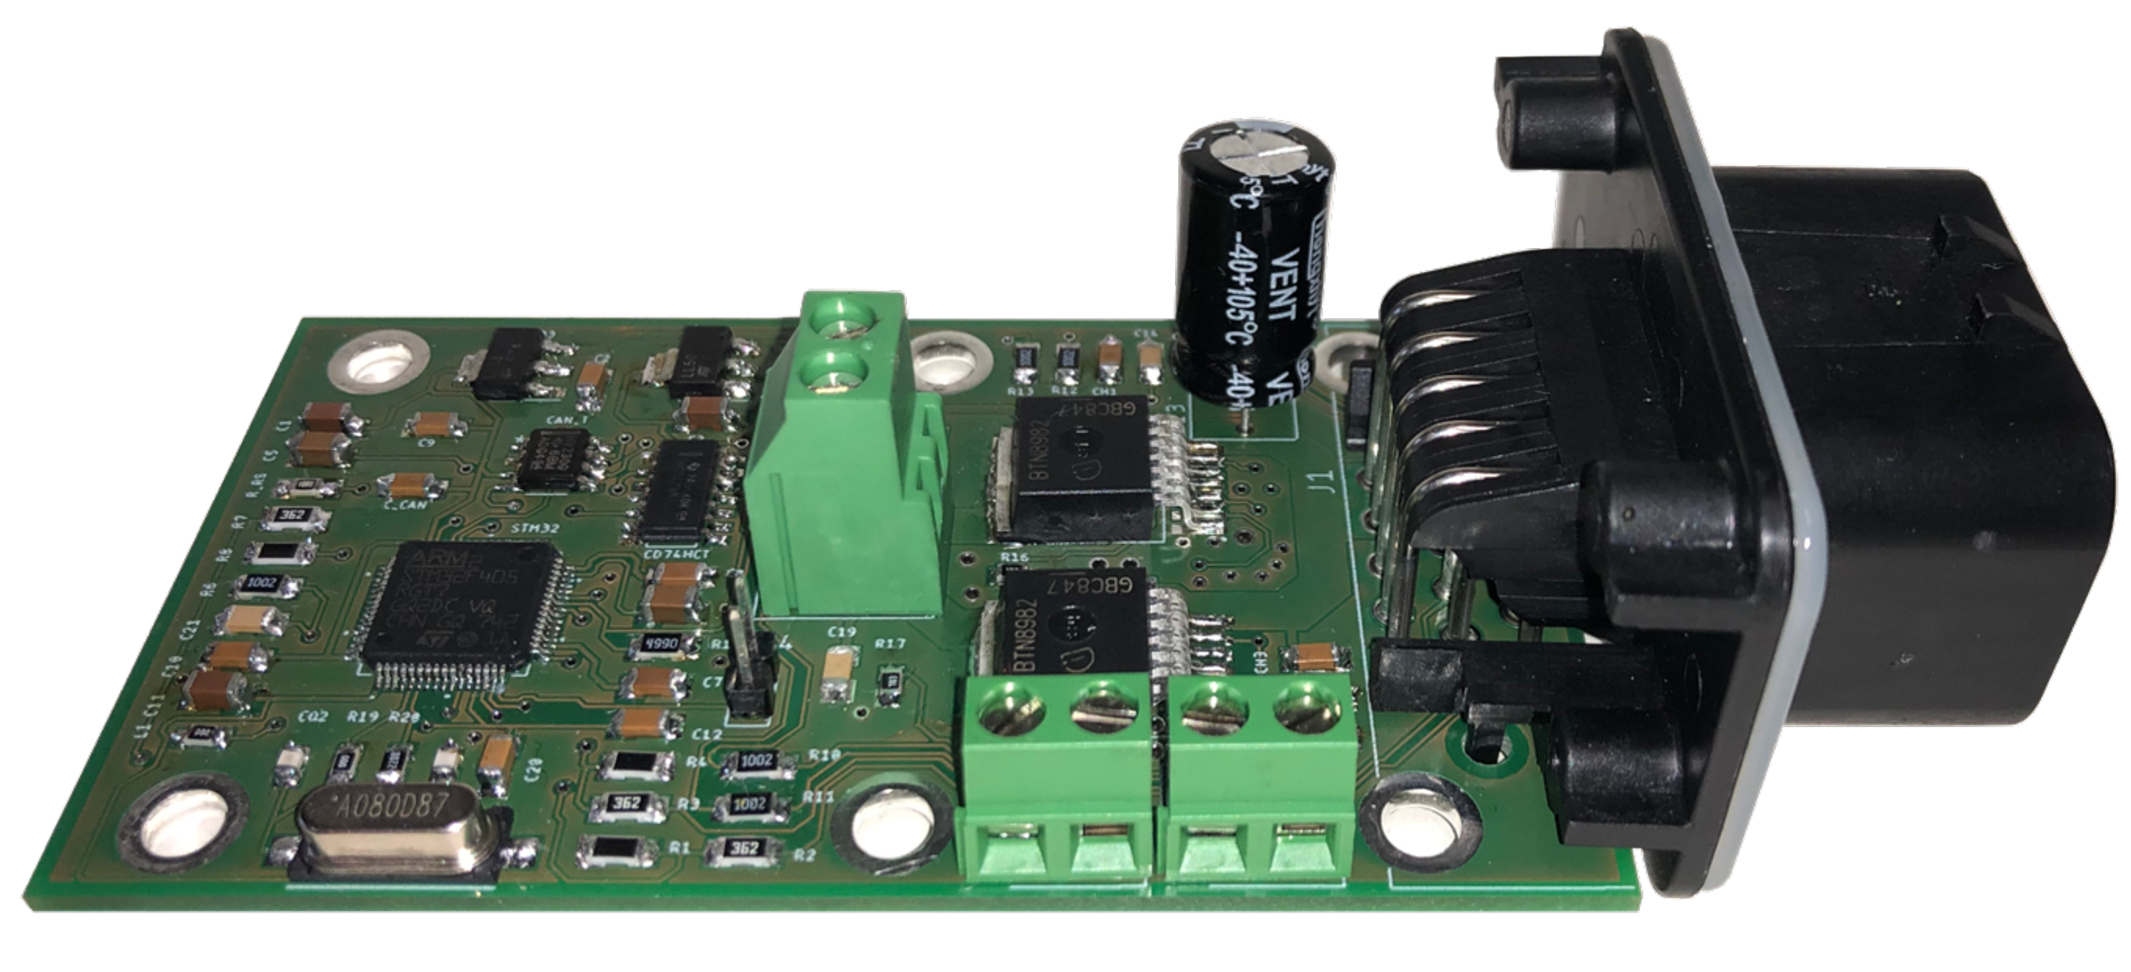
\includegraphics[width=220pt]{./Bilder/Endprodukt}
\caption{Die fertig bestückte Platine}
\label{fig:endprodukt}
\end{figure} \noindent
Nachdem der Mikrocontroller einmal \textit{geflasht} wird, steht die Funktionalität bei anliegender Versorgungsspannung bereit. Die CAN-Schnittstelle der Platine stellt eine Echtzeitkommunikation mit der MicroAutoBox her, sodass der Aktor über die Benutzeroberfläche ControlDesk am PC gesteuert werden kann. Die H-Brückenschaltung ermöglicht das Ansteuern des Aktors und somit das Schalten des Getriebes in Normalstellung oder einen der beiden Gänge. Der Lagesensor erfasst währenddessen die Position der Schaltgabel, die über die nichtflüchtige Kalibrierung genau berechnet werden kann. Die implementierte Regelung sorgt für die möglichst genaue Einhaltung der Sollvorgabe der Schaltgabelposition.
In der vorliegenden Arbeit konnte eine funktionierende eingebettete Elektronik für den linearen Tauchspulenaktor am Prüfstand des IMS entwickelt werden. Besonders hervorzuheben ist dabei die Kompaktheit der Platine, die direkt am Aktor angebracht wird, gegenüber dem vorherigen Zustand. In \autoref{fig:vergleich} wird das Endprodukt dem Arduino IBT2 Motortreiber gegenübergestellt. Der Größenvergleich zeigt, dass die Platine nur ungefähr doppelt so groß ist, dabei aber deutlich mehr Komponenten integriert hat.
\begin{figure}[H]%
\centering
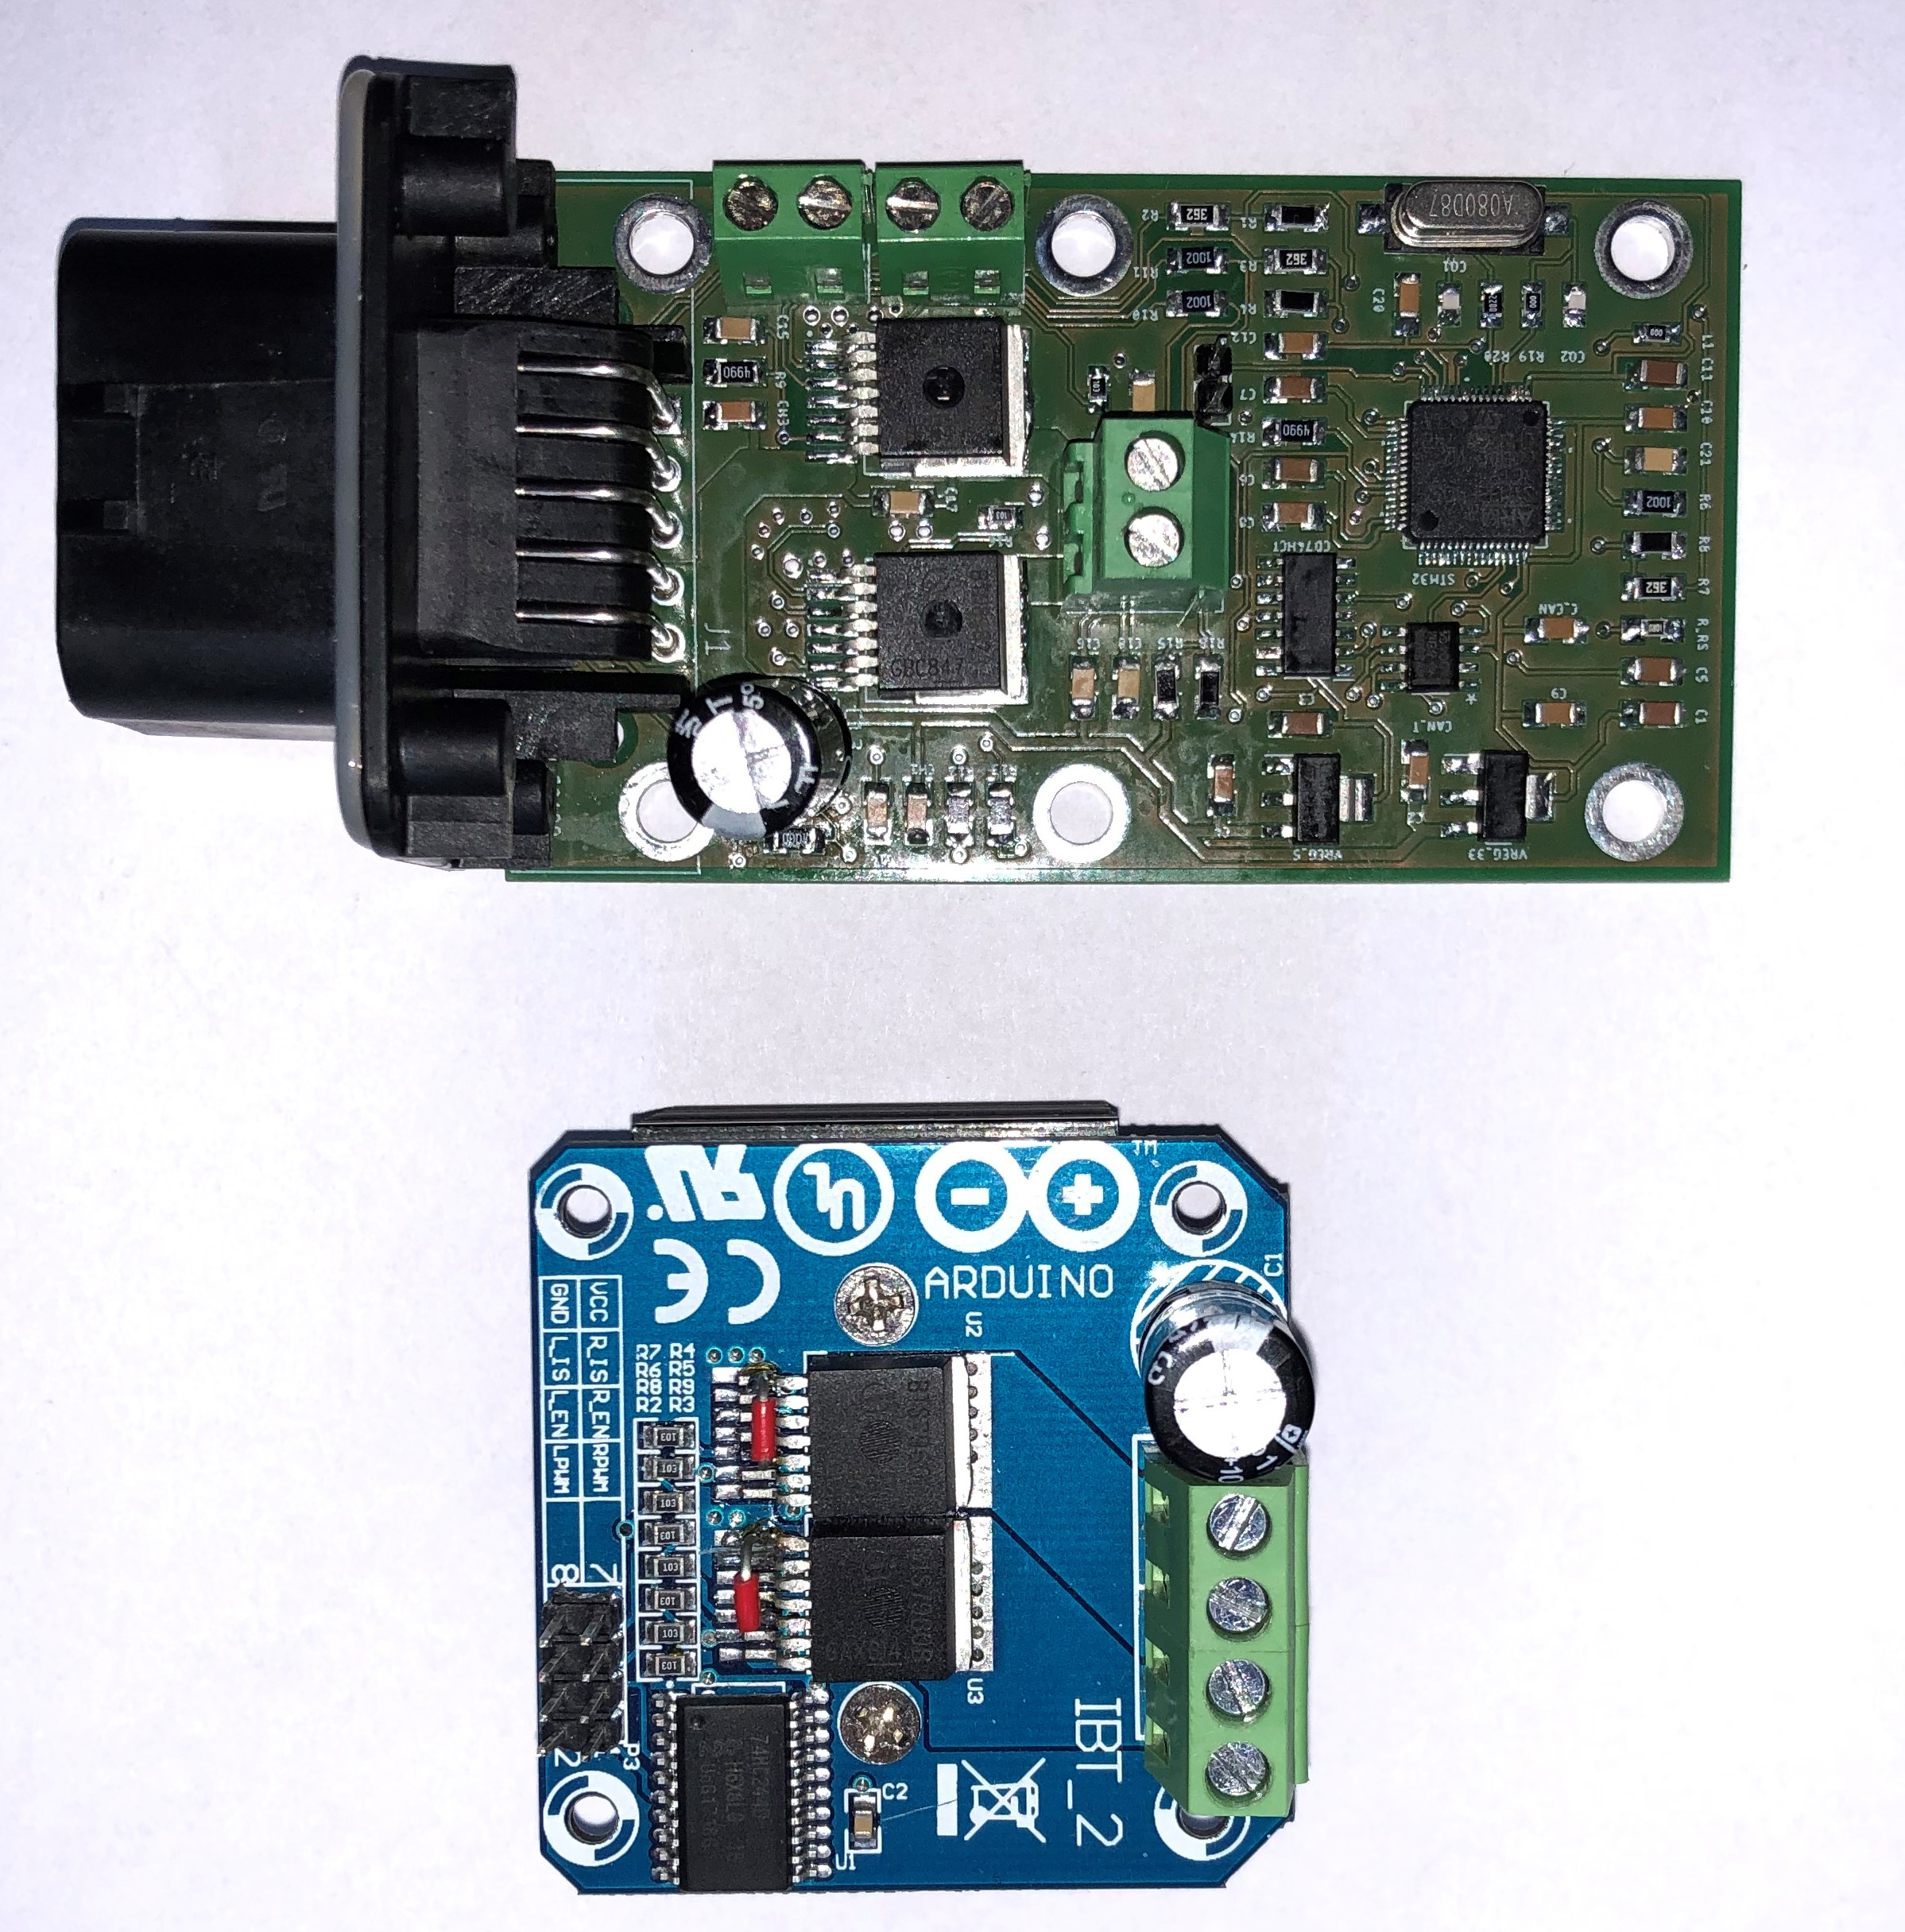
\includegraphics[width=0.35\columnwidth]{./Bilder/VergleichPlatine}%
\caption{Größenvergleich des Endprodukts mit IBT2 Motortreiber}%
\label{fig:vergleich}%
\end{figure}
Schnittstellen sowie Versorgung sind über einen einzigen Steckerausgang verbunden, der wahlweise mit dem passenden Gegenstück zur Programmierung oder zum Betrieb gekoppelt werden kann. 
\autoref{fig:platineaktor} zeigt auf der linken Seite die Platine in ihrem Elektronikgehäuse, welches an den nebenliegenden Aktor montiert wird. In der rechten Darstellung ist Platine samt Gehäuse und neuem Aktor zu sehen, wie das System später am Prüfstand angebracht wird. Auch der alte Aktor ist links daneben zu sehen.
\begin{figure}[H]
\centering
\includegraphics[width=480pt]{./Bilder/Platinefertig}
\caption{Anbringung der Platine in ihr Gehäuse und an den Aktor}
\label{fig:platineaktor}
\end{figure}
Die gestellten Anforderungen wurden weitestgehend erfüllt (vgl. \autoref{vergleich}), sodass von einem erfolgreichen und zufriedenstellenden Produktdesign ausgegangen werden kann. Eine Weiterentwicklung der eingebetteten Elektronik kann aufgrund der flexiblen Systemintegrierbarkeit und des leicht zu bedienenden Programms in weiteren Arbeiten erfolgen. 

\section{Ausblick} 

Der Schaltaktorikprüfstand des IMS wird stetig weiterentwickelt. So sind auch im Anschluss an diese Projektarbeit weitere Schritte zur Optimierung des Gesamtsystems denkbar und geplant. Zunächst soll der bisher angebrachte Aktor durch einen im Wirkprinzip äquivalenten Aktor mit einem Strom von ca. \SI{50}{A} bei maximal anliegender Spannung anstatt den jetzigen ca. \SI{19}{A} bei Maximalspannung ersetzt werden. Diese geplante Neuerung wurde auch in der Komponentenauswahl während dieser Arbeit  berücksichtigt, weshalb die Funktionalität der eingebetteten Elektronik auch weiterhin gegeben sein sollte. Weiterhin geplant ist es, die MicroAutoBox als CAN-Kommunikationspartner langfristig auszutauschen.
Das Mitschwingen des kompletten Prüfstands während den Kraftübertragungen eines Schaltvorgangs stellt ein Problem dar, welches die Messungenauigkeiten bedingen könnte. 
Sinnvoll wäre es, die Halterung des PLCD-Sensors zur Erfassung der Schaltgabelposition steifer zu gestalten, um eine optimale Positionsmessung und somit bessere Regelergebnisse zu erreichen. Bisher ist der Sensor leicht beweglich befestigt und kann sich somit schnell verstellen. Eine weitere Lösung für dieses Problem ist der Einsatz einer sensorlosen Positionserfassung, wie sie bereits in einer vorangegangenen Arbeit \cite{adp} theoretisch entwickelt wurde. Damals konnte die Umsetzung noch nicht erfolgen, da das Messverfahren nur auf der MicroAutoBox implementiert war, dessen Abtastrate des AD-Wandlers nicht hoch und die Anstiegsrate der digitalen Ausgänge zur Erzeugung einer PWM-Frequenz nicht schnell genug waren. Der STM32F405RGT7 mit einer ADC Abtastrate von bis zu 6Ms/s im Interleave Mode und einer Ansprechzeit von 125 ns ist laut den gestellten Anforderungen aber ausreichend, um das entwickelte Messverfahren durchzuführen.\\
Wie in \autoref{diskreg} analysiert wäre die Implementierung eines Haltereglers Gegenstand zukünftiger Forschung. Über diesen ließen sich eine Optimierung der Ganghaltung ermöglichen. 

